\chapter{Access Points}

The first main component of the Wi-Fi positioning system is the configuration
of the Access Points. In this chapter we describe how an AP works and how to
configure it.

\section{Linked list of the UEs}

First of all, the AP needs a data structure in order to save the different
measures of each User Equipment.

\subsection{Internal data structure}

Since UE measurements can be described as a simple structure containing only
two attributes -- the RSSI value and when this value has been retrieved -- its
seemed to be obvious to use a linked list.

\paragraph{}
The timer gives the AP the ability to delete a sample after a certain amount of
time which ensures to only keep accurate new values.

\paragraph{}
It becomes natural that the list is composed of elements where each of them
contains the MAC address of UE and a sample as shown below:

\begin{figure}[H]
  \centering
  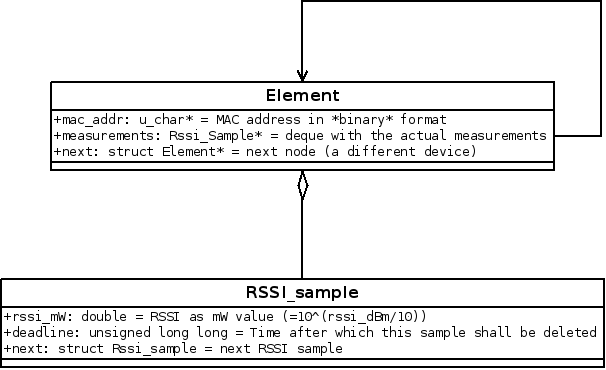
\includegraphics[scale=.6]{./ap/ap_list.png}
  \caption{Simplified linked list that each AP uses.}
\end{figure}

\subsection{Keep it up-to-date}

In the previous section, we quickly presented the timer attribute of an UE
measurement. We now go deeper and show why this is important.

\paragraph{}
Since an UE is moving all the time -- walking, going from the door to the
window, etc. -- keeping its measurements for too long will distort its
localization.

\paragraph{}
Therefore, in order to ensure the best possible accuracy, each measurement has
a timer and as soon as it reaches a life-span higher than a second, it is
removed from the list.

\paragraph{}
It is possible to constantly remove the old measurements using a daemon thread
that checks the `deadline` attribute of a list element as shown below:

\begin{figure}[H]
  \centering
  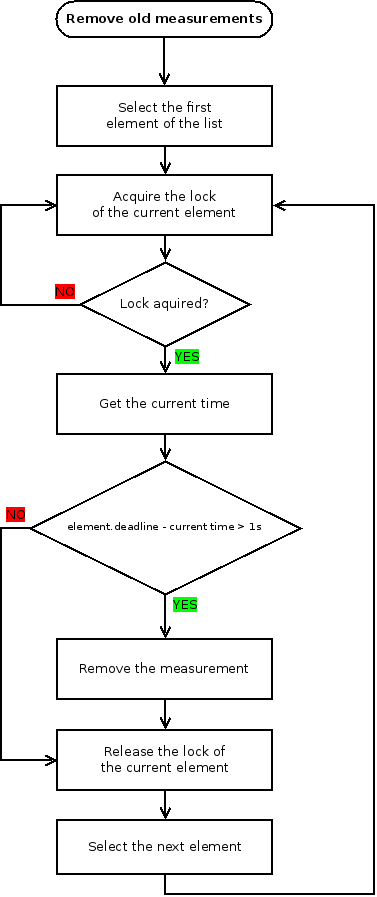
\includegraphics[scale=.7]{./ap/ap_list_thread.png}
  \caption{Remove old measurements in the list.}
\end{figure}

Due to a lack of time, we were not able to complete the implementation of this
feature in our project.

\subsection{Build the response}

In order to prepare the communication between the AP and the Positioning
Server, the AP list also gives a function that will convert the list into a
JSON formatted response.

\paragraph{}
Named `build\_buffer`, this function looks for a specific MAC address in the
list. It then retrieves the RSSI values the AP has and computes their average
value.

\paragraph{}
Then, using the `snprintf` standard C function, it converts the result into a
JSON dictionary, fully prepared to be sent back to the PS.

\section{Passive Sniffer}

We have seen how the AP stores the data. Let us now see how it finds each
value.

\subsection{Listen to Wi-Fi packets}

In order to find the MAC addresses and the RSSI values of each device, it needs
to sniff the network for any Wi-Fi signals sent by the UEs. The AP achieves
this sniffing by using the \emph{PCAP} library.

\paragraph{}
It sets up a hook on its wireless interface in order to intercept any
Wi-Fi packets on the network like shown in the scenario below:

\begin{figure}[H]
  \centering
  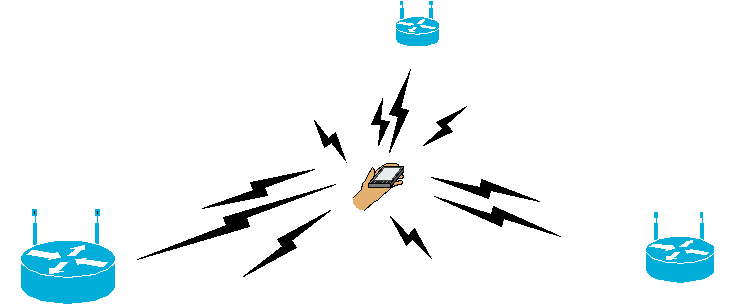
\includegraphics[scale=.5]{./ap/mobile_with_aps.png}
  \caption{Each AP sniffs the Wi-Fi packets of the network.}
\end{figure}

\subsection{Extract the values}

Then for each packet, it extracts the MAC address and the RSSI value fields and
stores them into its list.

\begin{figure}[H]
  \centering
  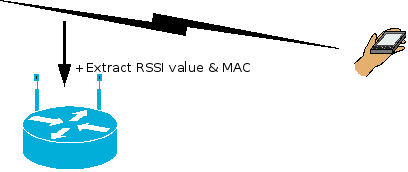
\includegraphics[scale=.7]{./ap/focus_mobile_with_aps.png}
  \caption{For each packet, the AP extracts two fields.}
\end{figure}

\paragraph{}
For some times, we had a bug when using the \emph{PCAP} library. The sneakiest
problem we have met occurred because of the version the \emph{PCAP} library
that was running on the AP.

\paragraph{}
Indeed, for some versions, a field was added in the header and triggered a
buffer overflow when trying to retrieve the different informations we were
looking for.

\section{HTTP Daemon}

Last but not least, the AP needs a way to communicate with the PS. This section
describes how we manage to set up a communication system between both.

\paragraph{}
At this point, the AP is able the measure every RSSI values for any devices on
the network and stores them. It is also able to convert them to a JSON
formatted dictionary.

\paragraph{}
So in order to send that dictionary to the PS, we have set up a HTTP daemon
using the \emph{MicroHTTP} library.

\paragraph{}
When being fired up, it initializes that daemon using the
\emph{start\_microhttpd} function. As a callback function, the AP passes the
\emph{connection\_callback} one that reacts to any \emph{?mac=} HTTP requests.

\paragraph{}
Hence the AP is now able to communicate with the PS. The
\emph{connection\_callback} is triggered each time the server asks the
measurements of an UE. It then processes the list and builds the response.

\section{Run the program}

We now have every parts of the AP -- a data structure, a sniffer and a HTTP
daemon -- except how to configure and install it on the AP itself. This section
answers theses questions.

\subsection{Configuration}

The only configuration our project requires concerns the HTTP daemon and the
interface on which to set up the sniffer.

\paragraph{}
The \emph{http\_daemon.h} file defines two constants:

\begin{enumerate}
    \item The port on which the daemon will listen to. By
        default it is set to \emph{8080}
    \item The MAC address of the AP.
\end{enumerate}

\paragraph{}
Then the interface can be set up in the \emph{main.c} file.

\subsection{Installation}

Then, in order to create the program, we provide a \emph{Makefile} along with
the source files. Using the command \emph{make all} will generate the binary
(it requires the \emph{OpenWRT} toolchain).

\paragraph{}
Then the binary has to be copied onto the AP (using the \emph{scp} command for
instance).

\paragraph{}
Last, the command \emph{./ap\_daemon.bin} as to be run in order to run the
binary on the AP.
